%==============================================================
% Part 1 : The introduction 
%==============================================================
\let\rbackup\r
\newcommand{\x}{{\mathbf{x}}}
\renewcommand{\u}{{\mathbf{u}}}
\newcommand{\w}{\mathbf{w}}
\newcommand{\y}{{\mathbf{y}}}
\newcommand{\bx}{\x}
\newcommand{\bu}{\u}
\newcommand{\bv}{v}
\newcommand{\btau}{\tau}
\newcommand{\by}{{\tilde\y}}
\newcommandx{\xb}[2][1=n,2=k]{\x_{#1|#2}}
\newcommandx{\ub}[2][1=n,2=k]{\u_{#1|#2}}
\newcommandx{\wb}[2][1=n,2=k]{\w_{#1|#2}}
\renewcommand{\r}{\mathbf{r}}
\newcommand{\rx}{\r^\x}
\newcommand{\ru}{\r^\u}
\newcommand{\vv}{{{v}}}
\newcommandx{\gb}[3][1=n,2=k,3={}]{g_{#1|#2}^{#3}}
\newcommandx{\hb}[3][1=n,2=k,3={}]{h_{#1}^{#3}}
\newcommandx{\vb}[2][1=n,2=k]{\vv_{#1|#2}}
\newcommandx{\tb}[2][1=n,2=k]{\tau_{#1|#2}}
\newcommand{\blambda}{{\boldsymbol{\lambda}}}
\newcommand{\bmu}{{\boldsymbol{\mu}}}
\newcommand{\rr}{{\mathrm{r}}}
\newcommand{\ff}{\mathrm{f}}
\newcommand{\bxi}{{\boldsymbol{\xi}}}
\newcommand{\bet}{{\boldsymbol{\nu}}}
\newcommand{\ped}{\mathrm{ped}}
\newcommand{\rped}{\r^\ped}
\newcommand{\rxped}{\r^{\x,\ped}}
\newcommand{\ruped}{\r^{\u,\ped}}

\newcommand{\matr}[2]{\left[\begin{array}{#1}#2\end{array}\right]}

\chapter{Introduction}\label{chapter:intro}
The way of transportation is in a transformation phase and autonomous driving technology is expected to have a big impact. Over one million people are killed in traffic-related accidents each year, where the vast majority of the accidents are caused by human mistakes~\cite{WHO2018, NHTSA2018}. 

Autonomous driving technology is expected to have a massive effect on the current transportation system and benefit society in many ways. For example, over one million people are killed in traffic-related accidents each year, where the vast majority of the accidents are caused by human mistakes~\cite{WHO2018, NHTSA2018}. By removing humans from the control of the vehicles, autonomous driving could significantly improve the traffic safety. Furthermore, the productivity of commercial heavy vehicles is increased when fewer human drivers are required, and the road infrastructure could be utilized more efficiently by scheduling transports outside of rush hours, for example during nights~\cite{FAGNANT2015167}.

Major progress towards deploying autonomous vehicles has been made during the last decade. The perception systems have been remarkably improved, largely due to the success of deep learning techniques~\cite{Janai2020}. The low-level control of the vehicle is a mature research area and can be solved with classical control theory methods~\cite{Paden2016}. However, how to approach the high-level decision-making in complex traffic situations is less explored and forms the main topic of this thesis.

\section{Problem formulation}
The work presented in this thesis has in particular focused on the following research questions:
\begin{enumerate}
	\item[\textbf{Q1.}] How can RL be used to create a decision-making agent for autonomous driving, that can handle different intersection and roundabouts (complex urban scenarios)? Learn a scalable policy that is able to handle different scenarios. relative coordinate system. Action space. 
	(specificera for att komma undan varfor har du inte kollat pa andra metoder. How can we use RL for AD )
	\item[\textbf{Q2.}] How can AD domain knowlage (and models) be used to improve the action and state space for a RL agent? MPC for actions, Particle filter for intention distrubution. How can AD domain knowlage be used to create a state and action space that improves the RL agent?
	\item[\textbf{Q3.}] How can the quality of a RL agent be imporved by accounting for uncertainty?
	(How can the uncertainty of the RL agent be utilized?) (RPF-in the output and PF-in the input space)
\end{enumerate}



\begin{enumerate}
	\item We want to drive through intersections. 
	\item The intersection can be of different shapes. We assume we have a map of the intersection. 
	\item There will be other cars crossing the same intersection. 
	\item We have access to sensors on-board the ego vehicle. 
	\item We dont assume any knowlage of traffic signs or traffic lights. 
	\item We dont have v2v, or v2x communication. 
	
	To compensate for not having v2v or v2x communitaion, we have to predict what other driver will do. 
	
\end{enumerate}



\section{Scope and limitations}
FILL

\section{System architecture}
outline system architecture and limit this papre to comfortable decisions \gls{rl}

\begin{figure}[t]
	\centering
	\mbox{\parbox{\textwidth}{
			\centering
			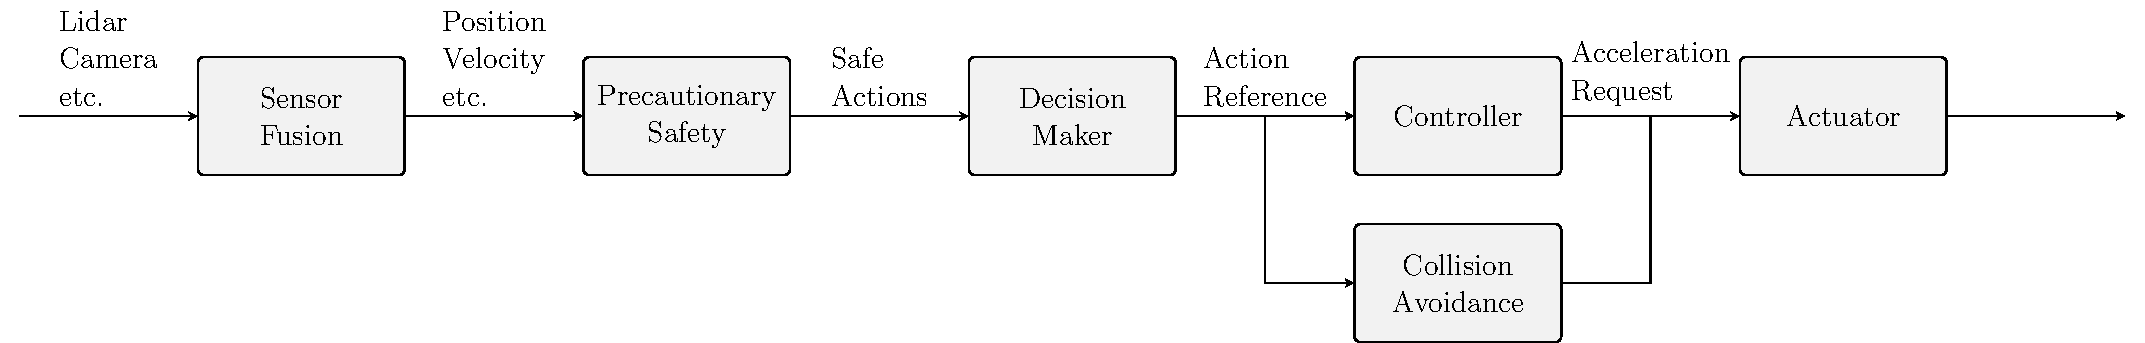
\includegraphics[width=\linewidth]{YourThesis/chapters/figures/pomdp/figures-system_architecture.pdf}%We suggest that you use a text box to insert a graphic (which is ideally a 300 dpi TIFF or EPS file, with all fonts embedded) because, in an document, this method is somewhat more stable than directly inserting a picture.   
	}}
	\caption{Representation of the system architecture.
	}
	\label{fig:system_architecture}
\end{figure}

\section{Contributions}

The main contributions of this thesis are:
\begin{enumerate}
	\item FILL

\end{enumerate}


\section{Thesis outline}
FILL



% !TEX root=../../Thesis.tex
\chapter{Technical Background}\label{chapter:background}
%

\section{Partially Observable Markov Decision Process}\label{section:pomdp}

\begin{itemize}
    \item POMDP
    \item State - realative features, scalable to fidderent types of intersection design 
    \item Action - IDM - MPC
    \item Observation - unknown intentions, red lights, stop signs yield. 
    \item Transistion function - RL 
    \item Reward Function - Goal, Comfort, crash
    \item discount factor 
\end{itemize}

\chapter{Technical background}
\label{ch:theoreticalBackground}

% Now not using time index, e.g., s_t. Check if consistent with subsequent chapters.
%    - Time index not used (much) in Paper 2-5, but in Paper 6. Slighlty inconsistent at the moment, but doesn't matter too much...

% This chapter gives a brief introduction to
% %how the problem of making sequential decisions based on uncertain information can be modeled, 
% Markov decisions processes
% and reinforcement learning. Notation that is used in subsequent chapters is also introduced. The material in this chapter is based on Kochenderfer~\cite{Kochenderfer2015} and Sutton et al.~\cite{Sutton2018}, which provide a comprehensive overview of MDPs and RL.

This chapter provides a brief introduction to Markov decision processes and reinforcement learning.
%, together with the notation that is used in subsequent chapters. 
% The reader who is familiar with these concepts could probably skip this chapter and return in case of any confusion concerning the notation. 
The purpose of the chapter is to summarize the most important concepts and introduce the notation that are used in the subsequent chapters. 
A comprehensive overview of MDPs and RL is given in the books by Kochenderfer~\cite{Kochenderfer2015} and Sutton and Barto~\cite{Sutton2018}, upon which this chapter is based.


\section{Markov decision processes}
\label{sec:mdp}
%MDP
Sequential decision-making problems in stochastic environments are commonly modeled as MDPs. Importantly, an MDP satisfies the Markov property, which requires that the probability distribution of the next state only depends on the current state and the action taken by the agent, i.e., not on the history of previous states or actions. An MDP is formally defined as the tuple $( \mathcal{S}, \mathcal{A}, T, R, \gamma )$, which is described in the following list~\cite[Ch. 4]{Kochenderfer2015}:
%
\begin{itemize}
    \item The state space $\mathcal{S}$ represents the set of all possible states of the environment. This set could consist of both discrete and continuous states.
    \item The action space $\mathcal{A}$ represents the set of all valid actions the agent can take. This set could also consist of both discrete and continuous actions. However, since this thesis focuses on high-level decision-making, only discrete actions are considered here.
    \item The state transition model $T(s'|s,a)$ describes the probability that the system transitions to state $s' \in \mathcal{S}$ from state $s \in \mathcal{S}$ when action $a \in \mathcal{A}$ is taken.
    \item The reward function $R(s,a)$ returns a scalar reward $r$ for each state-action pair.
    \item The discount factor $\gamma \in [0,1)$ is a scalar that discounts the value of future rewards. For a finite horizon MDP, $\gamma$ could also take the value~$1$.
\end{itemize}

A policy $\pi$ is a mapping from a state to an action, which could either be deterministic $a=\pi(s)$ or probabilistic $a \sim \pi(a|s)$. The value of being in a state while following a policy is described by the value function
%
\begin{align}
    V^\pi(s) = \mathbb{E} \left[ \sum_{k=0}^\infty \gamma^k R(s_k, a_k) | s_0 = s, \pi \right].
\end{align}
%
The goal of the agent is to find a policy which maximizes the value of each state.

% In this framework, an agent chooses an action $a$, based on the current state $s$, then receives a reward $r$, and transitions to a new state $s'$. An MDP satisfies the Markov property, which assumes that the probability distribution of the next state only depends on the current state and action, and not on the history of previous states. The MDP is defined as the tuple $( \mathcal{S}, \mathcal{A}, T, R, \gamma )$, where $\mathcal{S}$ is the state space, $\mathcal{A}$ is the action space, $T$ is a state transition model, $R$ is a reward model, and $\gamma \in [0,1]$ is a discount factor. 
% The state transition model $T(s' \mid s,a)$ describes the probability that the system transitions to state $s'$ from state $s$ when action $a$ is taken, and the reward model defines the reward of each step as $r=R(s,a,s')$.
% The goal of an agent is to find a policy $\pi(s)$ which for every time step $t$ chooses an action that maximizes the future discounted return $R_t$, defined as
% %
% \begin{align}
%     \label{eq:discountedReturn}
%     R_t = \sum_{k=0}^\infty \gamma^k r_{t+k},
% \end{align}
% %
% where $r_{t+k}$ is the reward at step $t+k$.


%POMDP
In many decision-making problems, the agent does not have direct access to the state of the environment. Such a problem is commonly modeled as a partially observable Markov decision process, which is an extension to the MDP framework that also models state uncertainty. A POMDP is formally defined as the tuple  $( \mathcal{S}, \mathcal{A}, \mathcal{O}, T, O, R, \gamma )$, where the state space, action space, transition model, reward function, and discount factor are defined as for an MDP. A POMDP has two additional components~\cite[Ch. 6]{Kochenderfer2015}:
%
\begin{itemize}
    \item The observation space $\mathcal{O}$, which is the set of possible observations.
    \item The observation model $O(o|s',a)$, which describes the probability of observing $o \in \mathcal{O}$ in state $s'$ after action $a$ has been taken.
\end{itemize}
%
Since the agent does not have direct access to the current state in a POMDP, the agent needs to reason about the history of observations and actions. This history is often merged in a belief state $b$, which represents a probability distribution over the state space. In this case, the policy is a mapping from beliefs to actions $\pi(b)$.



%In many decision-making problems, the exact state is not known by the agent and it only perceives observations $o$. A problem with state uncertainty can be modeled as a partially observable Markov decision process, which is defined by the tuple $( \mathcal{S}, \mathcal{A}, \mathcal{O}, T, O, R, \gamma )$. Compared to an MDP, the POMDP includes an additional observation space $\mathcal{O}$, and an observation model $O(o \mid s,a,s')$, which describes the probability of observing $o$ in state $s'$, after taking action $a$ in state $s$.


For many real-world problems, it is not possible to represent the probability distributions $T$ or $O$ explicitly. For some solution approaches, only samples are needed, and then it is sufficient to define a generative model $G$ that samples a new state or observation from a given state and action, i.e., $s' \sim G(s,a)$ for the MDP case~\cite[Ch. 4]{Kochenderfer2015} and $(s', o) \sim G(s,a)$ for the POMDP case~\cite[Ch. 6]{Kochenderfer2015}.


\section{Reinforcement learning}
\label{sec:rl}

If all the elements $( \mathcal{S}, \mathcal{A}, T, R, \gamma )$ of an MDP are known, an agent can use this model to directly compute an optimal policy. Such a problem is often considered a planning problem. For small MDPs, dynamic programming\footnote{Dynamic programming refers to simplifying a complex problem by breaking it down into smaller sub-problems, often in a recursive manner.} techniques can provide an exact solution, which is calculated offline, i.e., before the agent is deployed in the environment. For example, in value iteration~\cite[Ch. 4]{Kochenderfer2015}, the Bellman operator is iteratively applied to the value function for all states,
%
\begin{align}
    V_{n+1}(s) = \max_a \left[ R(s,a) + \gamma \sum_{s'}T(s'|,a,s)V_n(s') \right].
\end{align}
%
As $n$ goes to infinity, $V_n$ converges to the unique optimal value function $V^*$, and an optimal policy (not necessarily unique) is extracted by
%
\begin{align}
    \pi(s) = \argmax_a \left[ R(s,a) + \gamma \sum_{s'}T(s'|,a,s)V^*(s') \right].
\end{align}
%
However, for many real-world problems with high dimensional state spaces, it is intractable to compute and store a policy offline. Contrarily to offline methods, online search methods perform planning from the current state up to some horizon, when the agent has been deployed. Thereby, the agent can limit the computation to states that are reachable from the current state, which is often significantly smaller than the full state space~\cite[Ch. 4]{Kochenderfer2015}.

% \begin{figure}[!bt]
%     \centering
%         \vspace{-10pt} % To avoid widow word.
%         \includegraphics[width=0.7\columnwidth]{figures/RL_cropped.pdf}
%         \caption{In a reinforcement learning problem, an agent learns a policy $\pi$ by interacting with its environment. The agent collects experience by repeatedly taking actions and then observing the resulting state and reward.}
%         \vspace{-10pt} % To avoid widow word.
%     \label{fig:RL}
% \end{figure}

In many problems, the state transition probabilities or the reward function are not known. These problems can be solved by reinforcement learning techniques, in which the agent learns how to behave from interacting with the environment~\cite[Ch. 5]{Kochenderfer2015}, see Figure~\ref{fig:RL}. Compared to supervised learning, reinforcement learning presents some additional challenges. Since the data that are available to an RL-agent depends on its current policy, the agent must balance exploring the environment and exploiting the knowledge it has already gained. Furthermore, a reward that the agent receives may depend on a crucial decision that was taken earlier in time, which makes it important to assign rewards to the correct decisions.

%If MDP is known, planning. RL deals with unknown T or G, interacts with environment to learn. Figure.
% As mentioned above, the goal of a decision-making agent is to take actions that maximizes the future discounted return $R_t$. If all elements of the MDP are known, the agent could compute which action that is ideal before executing any actions in the environment, which is referred to as planning. However, in many problems the transition model or generative model is not known to the agent beforehand and it needs to learn how to behave from experience, which is referred to as a reinforcement learning problem. The agent will then act in the environment and observe what happens, in order to figure out a policy $\pi$, which defines which action to take in a given state.
% Figure~\ref{fig:RL} shows a schematic overview of the reinforcement learning problem.
% The agent is commonly represented by a neural network, which acts as a nonlinear function approximator. Further details on neural networks and how they can be used in RL are described by Sutton et al.~\cite{Sutton2018}.


%Reinforcement learning is a class of machine learning techniques, which enables an agent to learn a policy $\pi$ that maximizes the expected future return $\mathbb{E}(R_t)$ in the environment the agent acts in~\cite{Sutton1998}. 



%Model based vs model-free
% Model based - learns model T, then planning
% Model free - does not learn model
% Model free techniques range from direct policy search vs value-based RL

%One approach to decide which action to take is to first try to learn the model of the environment from the observations, i.e., to learn $T$. Once the model is learned, a planning algorithm could be used to find the best policy. RL approaches that follows this structure are called model based RL algorithms.

RL algorithms can be divided into model-based and model-free approaches~\cite[Ch. 5]{Kochenderfer2015}. In the model-based versions, the agent first tries to estimate a representation of the state transition function $T$ and then use a planning algorithm to find a policy. On the contrary, as the name suggests, model-free RL algorithms do not explicitly construct a model of the environment to decide which actions to take. 
The model-free approaches can be further divided into value-based and policy-based techniques. Value-based algorithms, such as $Q$-learning, aim to learn the value of each state and thereby implicitly define a policy. Policy-based techniques instead search for the optimal policy directly in the policy space, either by policy gradient methods or gradient-free methods, such as evolutionary optimization. There are also hybrid techniques that are both policy and value-based, such as actor critic methods.


% Genetic algorithms belong to a family of optimization methods that are inspired by the evolutionary mechanisms of natural selection~\cite{Holland1975}.
% In general, GAs are suitable for solving optimization problems where the objective function is non-differentiable, or even when an explicit mathematical model does not exist and only a simulation is available. 
% A GA can also solve some versions of RL problems, and is used as an RL method in this thesis.


RL algorithms generally assume that the environment is modeled as an MDP, i.e., that the state of the environment is known by the agent. However, in many cases of interest, only partial information about the state of the environment is available, which is modeled in the POMDP framework. For such cases, it is common to approximate the state by either the observation or a finite history of observations~\cite[Ch. 17]{Sutton2018}. The latter is referred to as a $k$-Markov approximation, where $k$ defines the length of the included history. For a sufficiently long history, the Markov property is assumed to approximately hold, even though the environment is partially observable.

% Possibly add something about neural networks as function approximators somewhere in this section?
%    - No

\includepapersummary % Label: 'chap:papersummary'. Replace with separate file if the auto-generated summary does not work with your content.

\chapter{Concluding Remarks and Future Work}
\label{sec:conclusion}
%
% Q1. What requirements need to be set on the sensor-suite and prediction
% algorithms in order to enable safe autonomous driving?
% Q2. How should a vehicle controller be designed in order for safety to be
% proven by design?
% Q3. Can a safe AD framework be deployed on a real test platform?

While trying to answer the three research questions presented in Section~\ref{chapter:intro}, this thesis introduced a set of different MPC formulations intended for AD applications. In particular, we introduced MPC in a general sense in Chapter~2, and discussed why the standard results available in the literature cannot be directly applied to ensure safety in AD applications.  

Indeed, in order for a self-driving vehicle to become safe, it must be able to sense and predict its surrounding environment. Chapter~3 therefore introduced an efficient pedestrian prediction model (\paperPedestrian{}) and specified a requirement on prediction properties (Assumption~\ref{a:unknown_constraints}) that proves to be fundamental in ensuring safety (research question Q1).

Assuming that the environmental prediction models have a specific structure, we then show that safety guarantees could be enforced by the introduction of a safe set (\paperSafe). In other words, designing an MPC controller that is safe by design is possible (research question Q2). However, since MPC is an optimization-based technique, and can in general be computationally demanding, we show in Chapter~4 that it is still possible to deploy a safe MPC framework in a real vehicle platform (\paperPlanner, \paperExp), while satisfying the safety guarantees in Theorem~\ref{theorem:safe} (research question Q3).


Even though this thesis presented an approach to ensure safety for AD applications, it is far from being a ``silver bullet'' that solves all problems related to autonomous driving. Therefore, we will next comment on some possible extensions and also outline future research directions.



\section{Future Work}
While the results in Theorem~\ref{theorem:safe} guarantee safety, i.e., recursive feasibility, of the controller, it does not prove asymptotic stability when the a-priori unknown constraints are active. A promising future research direction, can therefore be to first expand the ISS results from \paperISS{} to general nonlinear systems, and then show some sort of ISS results also for Theorem~\ref{theorem:safe} by considering the road users as an input. Furthermore, while \paperISS{} showed that using infeasible references can still yield some stability results, it may be quite limiting to always use a pre-defined reference trajectory. To that end, it would also be interesting to combine the proposed framework with some form of re-planning or online learning, e.g., updating the reference velocity in the presence of road users that make the pre-defined reference infeasible.


\paperScenario{} showed that multi-modal prediction models could be used to improve the overall performance of the system. However, the results relied partly on the availability of such models, but also on a probability estimate for each predicted mode. Indeed, to be able to use these results more widely, a future direction would be to use some learning-based methods to estimate such probabilities from real data. In addition, since the predictability of the environment plays a large part in enabling safe autonomous driving applications, it is necessary to also direct research attention towards deriving models that can accurately represent the surrounding environment.


Finally, in order to further strengthen the results presented in this thesis, future work aims to implement the framework from \paperExp{} to a more general autonomous driving setting, where road users are not simulated, but measured and predicted in real-time.






%The predictability of the environment plays a large part in making safe autonomous driving applications a possibility. Indeed, being able to represent the surrounding environment in the least conservative, but most accurate way will enable the self-driving technology to progress even further. However, in order to so, some additional rules may need to be more clearly defined. For instance, prediction models that consider all worst-case behaviors will force a self-driving vehicle to drive slower than any human driver would, e.g., a conservative model that predicts that every pedestrian will intentionally run onto the road at all times will greatly limit the velocity at which the vehicle can drive, while always being able to capture the worst outcome. On the other hand, a model that predicts behaviors based on rules following from the legal road code may not model all pedestrians accurately. As such, this may require one to reason about a trade-off between performance and a willingness to take risks. Hence, new frameworks that ensure safety w.r.t a pre-specified risk-level may need to be considered instead.

%Future work aims to implement the safe MPC framework presented in Paper F in more complicated settings with actual road users and to verify the performance for more complicated settings.

% drive more cautiously than models that predict some nominal behavior that abides by a road code. However, it is clear that such a model



% For instance, one of the biggest 


% One of the most important aspects when it comes to 


% This thesis has discussed the importance of having consistent prediction models of the surrounding environment. 


% Concluding remarks
% % Lorem ipsum dolor sit amet, consectetur adipiscing elit, sed do eiusmod tempor incididunt ut labore et dolore magna aliqua. Ut enim ad minim veniam, quis nostrud exercitation ullamco laboris nisi ut aliquip ex ea commodo consequat. Duis aute irure dolor in reprehenderit in voluptate velit esse cillum dolore eu fugiat nulla pariatur. Excepteur sint occaecat cupidatat non proident, sunt in culpa qui officia deserunt mollit anim id est laborum.

% Lorem ipsum dolor sit amet, consectetur adipiscing elit, sed do eiusmod tempor incididunt ut labore et dolore magna aliqua. Ut enim ad minim veniam, quis nostrud exercitation ullamco laboris nisi ut aliquip ex ea commodo consequat. Duis aute irure dolor in reprehenderit in voluptate velit esse cillum dolore eu fugiat nulla pariatur. Excepteur sint occaecat cupidatat non proident, sunt in culpa qui officia deserunt mollit anim id est laborum.

% Lorem ipsum dolor sit amet, consectetur adipiscing elit, sed do eiusmod tempor incididunt ut labore et dolore magna aliqua. Ut enim ad minim veniam, quis nostrud exercitation ullamco laboris nisi ut aliquip ex ea commodo consequat. Duis aute irure dolor in reprehenderit in voluptate velit esse cillum dolore eu fugiat nulla pariatur. Excepteur sint occaecat cupidatat non proident, sunt in culpa qui officia deserunt mollit anim id est laborum.Lorem ipsum dolor sit amet, consectetur adipiscing elit, sed do eiusmod tempor incididunt ut labore et dolore magna aliqua. Ut enim ad minim veniam, quis nostrud exercitation ullamco laboris nisi ut aliquip ex ea commodo consequat. Duis aute irure dolor in reprehenderit in voluptate velit esse cillum dolore eu fugiat nulla pariatur. Excepteur sint occaecat cupidatat non proident, sunt in culpa qui officia deserunt mollit anim id est laborum.

%==============================================================